% ~~~ [ Control Flow Graph Generation ] ~~~~~~~~~~~~~~~~~~~~~~~~~~~~~~~~~~~~~~~~

\subsubsection{Control Flow Graph Generation}
\label{sec:design_control_flow_graph_generation}

The control flow graph generation component generates a CFG for each function of a given LLVM IR assembly file. As described in section~\ref{sec:lit_review_llvm_ir}, a function definition in LLVM IR consists of a set of basic blocks; and a basic block consists of zero or more non-branching instructions followed by a terminating instruction (such as \texttt{br} or \texttt{ret}) which changes the control flow. Therefore, the control flow graph generation component may focus on analysing the last instruction of each basic block, as they will determine the control flow.

To generate the CFG of a given function, a directed graph is created and populated with one node per basic block, and with zero or more directed edges between the nodes of the graph. The node names are determined by the basic block labels, and the directed edges are determined by the terminating instructions, as illustrated in figure~\ref{fig:directed_edges}.

\begin{figure}[htbp]
	\centering
	\begin{subfigure}[ht]{0.54\textwidth}
		\lstinputlisting[language=llvm, style=nasm, tabsize=2]{inc/8_ver/directed_edges.ll}
	\end{subfigure}
	\enskip
	\begin{subfigure}[ht]{0.22\textwidth}
		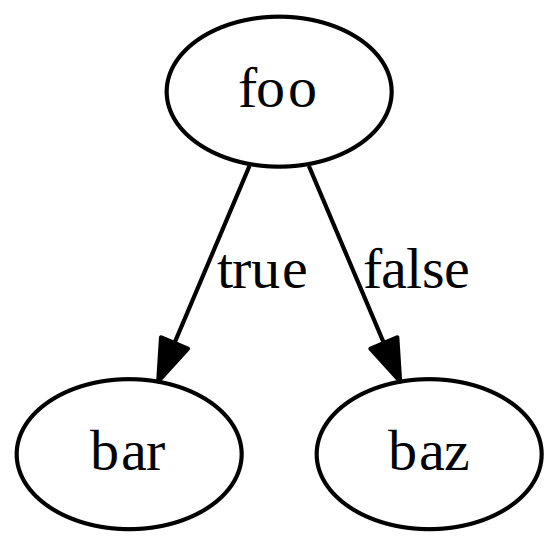
\includegraphics[width=\textwidth]{inc/8_ver/directed_edges.png}
	\end{subfigure}
	\caption{The return instructions of basic block \texttt{bar} and \texttt{baz} produces no directed edges, while the conditional branch instruction of basic block \texttt{foo} produces two directed edges in the CFG, one for each target branch (i.e. \texttt{bar} and \texttt{baz}).}
	\label{fig:directed_edges}
\end{figure}

The \texttt{ll2dot} tool generates CFGs from LLVM IR in the DOT file format, which is a well-defined textual representation of graphs used by the Graphviz project. One benefit of expressing CFGs in this format, is that the existing Graphviz tools may be facilitated to produce image representations of the CFGs; as demonstrated in appendix~\ref{app:control_flow_graph_generation_example}.
